%% sigconf for double column
%% natbib for bibtex
%% nonacm because it is not for a conference
\documentclass[format=sigconf, natbib=true, nonacm=true]{acmart}
\usepackage{lipsum}
\usepackage{hyperref}
\begin{document}
    \title{Impact on End-users by ISP IPv6 Deployment}

    \author{Tim Niklas Gruel}
    \affiliation{
    \institution{Ruhr-Universität Bochum}
    \city{Bochum}
    \country{Germany}
    }
    \email{tim.gruel@rub.de}

    \begin{abstract}
        This paper presents an overview of different techniques to cope with the IPv4 address exhaustion. The impact on the end-users is on focus. First some early NAT based solutions are introduced. Later dualstack is discussed. At the end IPv6 only solutions, deployed by ISPs today, are presented. It turns out that the end-user, especially the technical experienced one, can experience great benefits with IPv6. With IPv6 the internet gets back to its routs. All devices can talk to each other and central server are not mandatory anymore to establish communication.
    \end{abstract}

    \keywords{IPv6, Tunneling, Translation, End-user Impact, NAT64, DNS64, 464XLAT, Dualstack}

    %% page numbers
    \settopmatter{printfolios=true}

    \maketitle

    \section{INTRODUCTION}
    In the late 90s it became very clear, that the IPv4 address space is not sufficient to meet future demand. The popularity of the Internet especially in the end-user marked was heavily underestimated at the creation of IPv4. There are approximately 4 billion IPv4 addresses. Today there are over 8 billion humans on earth. That means that two humans need to share a single IPv4 address, not considering servers. Today, a typical family has multiple devices per person, including TVs, gaming consoles, smart phones, personal computers and many more. This led to the assignment of the last available IPv4 block in the early 2010s. With the rise of smart home technology and IoT devices, the demand for IP addresses per household will not stop to increase. In this paper I will present a nearly complete overview of the different ideas to slow down the inevitable IPv4 exhaustion. Expect for the last solution, none of these is a long term one or even tries to solve the problem itself. ISPs tried to keep cost as low as possible. This led to keeping IPv4 addresses as long as possible.\\\\First, ISPs started to assign only one public IP per customer. The customer had to use NAT44 in order to provide all his end devices with an internet connection. The end-user was the one getting a worse experience. Over time, assigning only one IPv4 per customer was too much for the ISPs. Especially with the rise of mobile internet and an even higher demand for addresses, IPv4 was doomed. ISPs tried to provide more IP addresses, by assigning only private IPv4 addresses to customers, leading to NAT444. NAT itself has many problems, which will be discussed in this paper. NAT444 makes the problems even worse. End-users were and are still heavily effected by that.\\\\A few years later dualstack was provided by ISPs. Dualstack introduced the next generation of IP addresses, called IPv6 addresses. Compared to IPv4 addresses which are a 32 Bit string, IPv6 addresses are a 128 Bit string. IPv6 completely solves the problem of address exhaustion. Unfortunately IPv6 is not backwards compatible to IPv4. Thus all infrastructure needs to be renewed. The Internet is fully decentralized. It is not possible to perform such a transition on one particular day. Dualstack implements both, IPv4 and IPv6. Devices and servers supporting IPv6 can communicate over IPv6. In the case that one device is not yet capable of IPv6, IPv4 acts as a fallback. This is a perfect transition technology, but it is no solution for the IPv4 exhaustion problem. Each end-user still needs an public or private IPv4. The problem is not solved.\\\\Lately, ISPs started to provide IPv6 only. This is also very common in mobile networks. The devices natively speak to servers over IPv6. For legacy IPv4 servers, there are different translation mechanisms. This paper will take a closer look into NAT64 combined with DNS64. Moreover I will present 464XLAT. Both are similar to a NAT44, but translating between IPv6 and IPv4. The interesting thing is that these translations happen at the ISP, so the end-user only uses with IPv6. This has many advantages for the end-user. Though, some legacy applications that depend heavily on IPv4 cannot be used. One example for that is Skype.\\\\At the end of this paper, tunneling IPv6 in IPv4 is presented. This happens only at ISP level and indirectly influences the end-user too. Mainly in better path availability, thus seamless internet service. There are many technologies. 6in4 and 6rd will be introduced shortly.\\\\In the last few years, the adoption of IPv6 has increased rapidly. On \url{https://www.google.com/intl/en/ipv6/statistics.html} it is possible to view the current adoption of IPv6 regarding the Google landing page. Germany for example has an adoption of over 65\%. This statistics really shows the trend of ISPs worldwide, deploying IPv6 only or dualstack. Nearly all mobile clients use IPv6 today and are able to interact with the Internet without notable disadvantages. Cisco predicts that the transition to IPv6 is finished in 2028. This means that nearly all end-users and servers world-wide communicate over IPv6. That has great advantages for the end-user regarding security and opens up entirely new options for innovative peer to peer technologies. Hosting a Server on a smart phone might sound strange today, but could be a very usual thing in 10 years from now. The end-user is the one benefiting the most from unique, world-wide routable IP addresses.\\\\Now I am going to turn back the time a bit and we are focusing on the problem, emerging in the late 90s. It becomes clear that the IPv4 address space is not big enough. ISPs are searching for a solution. The main goal is to assign the same public, globally routable IPv4 address to multiple devices. This is not meant for a long period of time, but much more as a quick fix, until the new standard IPv6 is developed.
    
    \section{EARLY SOLUTIONS}
    This section presents three different solution to extend the lifetime of IPv4. I will discuss NAT44, A+P and NAT444. All these solutions aim to share one single IPv4 address between multiple end devices. It is important to understand theses technologies in order to correctly estimate the impact of IPv6 deployment by ISPs. Evaluating modern solutions alone could lead to the impression, that these solutions are better or worse than they really are. Thus this paper starts with NAT44.
    \subsection{NAT44}
    NAT44 is also known as \textit{CPE NAT}. The word NAT stands for \textit{Network Address Translation}. \textit{NAT44} means that one IPv4 address is translated to multiple IPv4 addresses. CPE means \textit{Customer Premises Equipment}. The whole NAT procedure is up to the end-user. The ISP only provides one single IPv4 address. Typically one public, globally routable IP is translated to multiple private IP addresses. There are three private IPv4 Blocks which are the following:
    \begin{enumerate}
        \item 10.0.0.0/8
        \item 172.16.0.0/12
        \item 192.168.0.0/16
    \end{enumerate}
    Everybody can use the IPv4 addresses in these blocks. Private IPv4 addresses will never be routed in the internet. Most end-users use the third option for their home network. Thus they can use 254 different devices which is sufficient for most users. All these 254 devices share one public IPv4. All of them share the $2^{16} = 65536$ ports of the public IPv4 too. From the outside you cannot decide whether only one device or multiple devices are behind the NAT.
    \begin{figure}
        \centering
        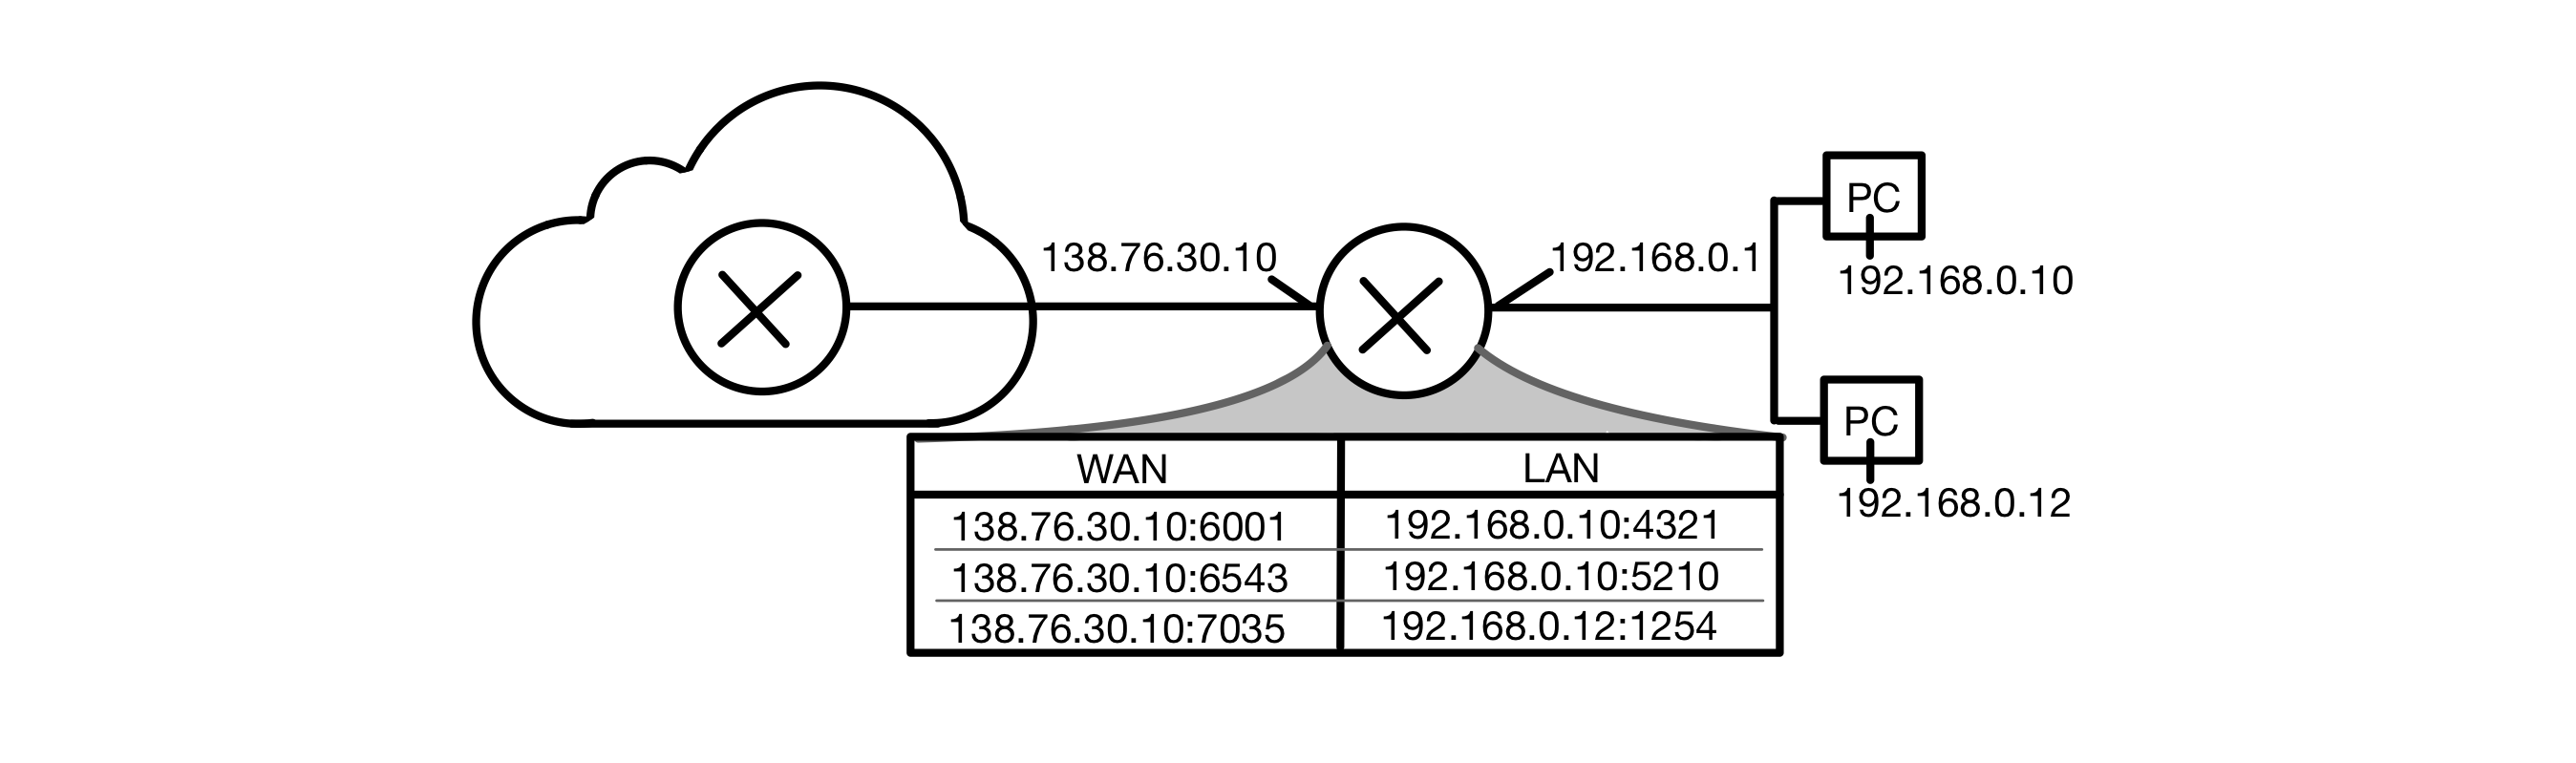
\includegraphics[width=0.5\textwidth]{images/nat_44.png}
        \caption{Example of NAT44 with NAT-Translation table}
        \label{fig:nat_44}
    \end{figure}
    In the example \ref{fig:nat_44} is a NAT-Translation table. As you can see, the PC with IP \textit{192.168.0.10} cannot use all ports, because the PC with the IP \textit{192.168.0.12} uses the Port \textit{7035}. All ports are shared. This can lead to problems as we discuss later. NAT44 was the first solution to the IPv4 exhaustion problem. It is an easy fix, because the ISP has nothing to change, except now only delivering one single IP per customer. The end-user needs a NAT compatible router.
    \subsection{A+P}
    \textit{A+P} means \textit{Address Plus Port}. Over the time NAT44 was not a sufficient solution anymore. The demand for IPv4 rose and ISP were not able to provide one single public, globally routable IPv4 per customer. The idea is still very similar to NAT44, but with \textit{A+P} each costumer gets one IPv4 and a designated port range. With that system it is possible to share one IP to theoretically \textit{65536} different customers \cite{8716482}.
    \begin{figure}
        \centering
        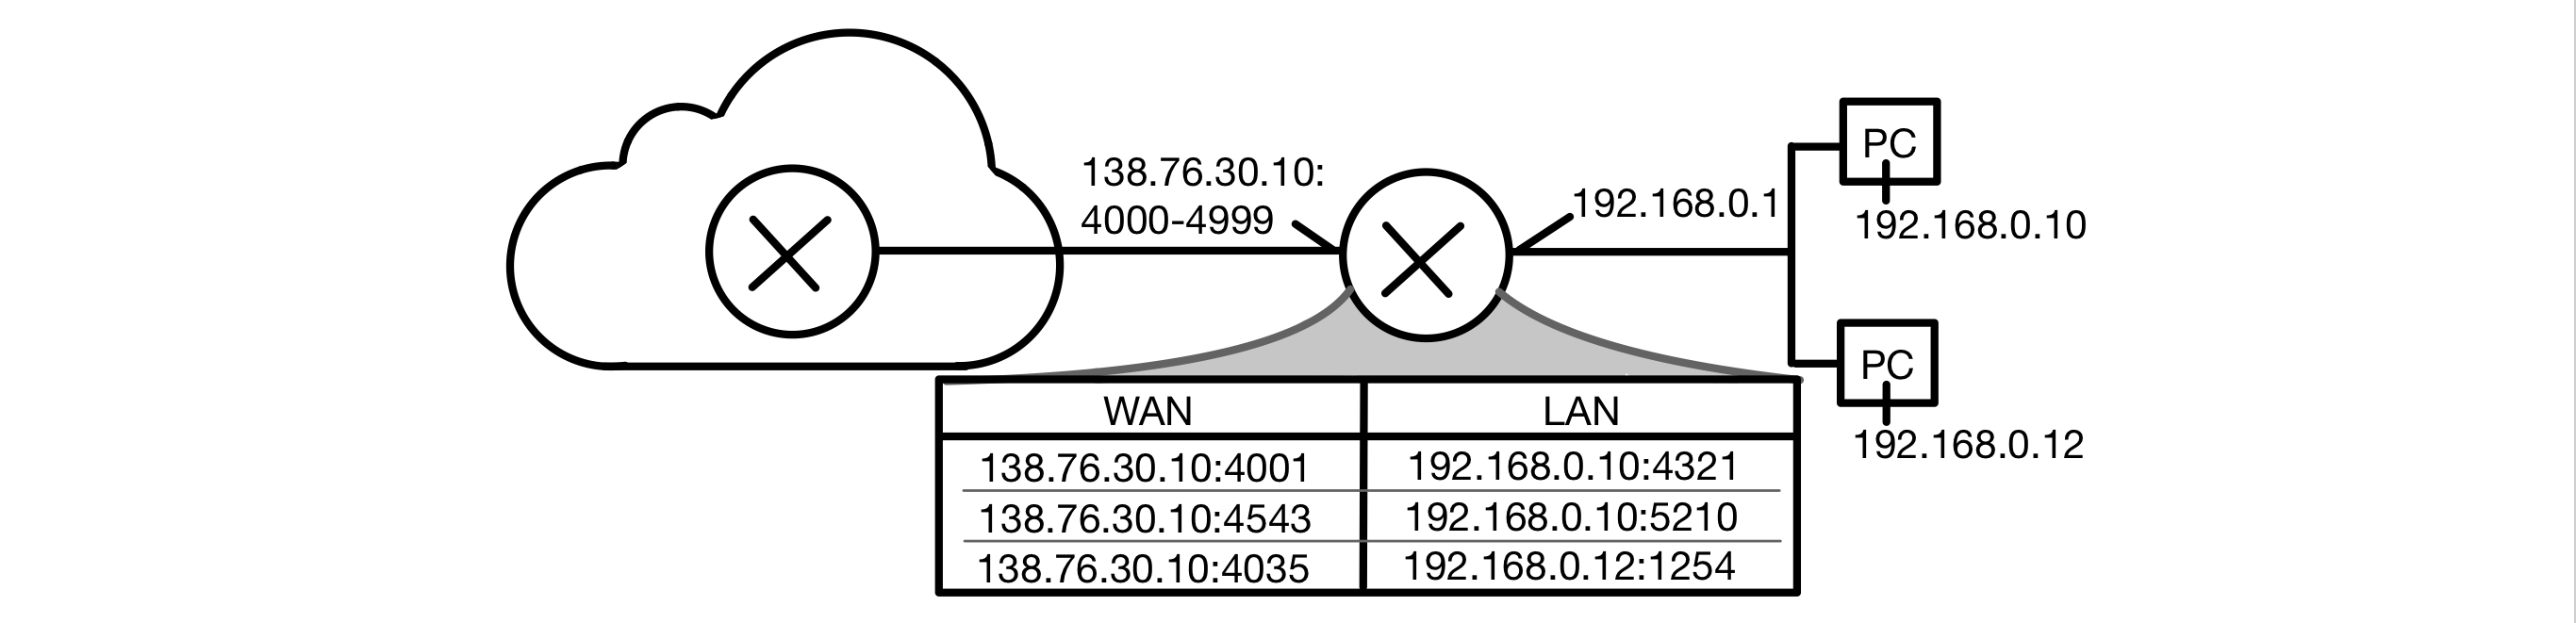
\includegraphics[width=0.5\textwidth]{images/a_plus_p.png}
        \caption{Example of A+P with NAT-Translation table}
        \label{fig:a_plus_p}
    \end{figure}
    In the example \ref{fig:a_plus_p} you can see that all internal ports are mapped to port values between \textit{4000} and \textit{4999}. This is because the ISP assigned this port range to that particular customer. All internal devices combined can open \textit{1000} ports. The biggest advantage of \textit{A+P} is also the biggest downside. On the one hand, it is possible to supply more customers with public, globally routable IPv4 address, but on the other hand all these customers have a tiny available port range. Assuming the extreme case of \textit{65536} different customers, each customer would only get one single port. Even when ports are dynamically assigned, the user experience at peak internet usage time would be unacceptable.
    \subsection{NAT444}
    \textit{NAT444} is also known as CGN. CGN means \textit{Carrier Grade Network Address Translation}. With NAT44 one public, globally routable IPv4 address is translated to multiple private IPv4 addresses at ISP site. Each customer gets one private IPv4 address. Similar to NAT44, the customer than translates that private IPv4 into multiple private IPv4 address for all home devices. That means there is a double NAT. IP addresses get translated twice \cite{10.1145/2987443.2987474}. This leads to even more problems than NAT44 or A+P \cite{8716482}.
    \begin{figure}
        \centering
        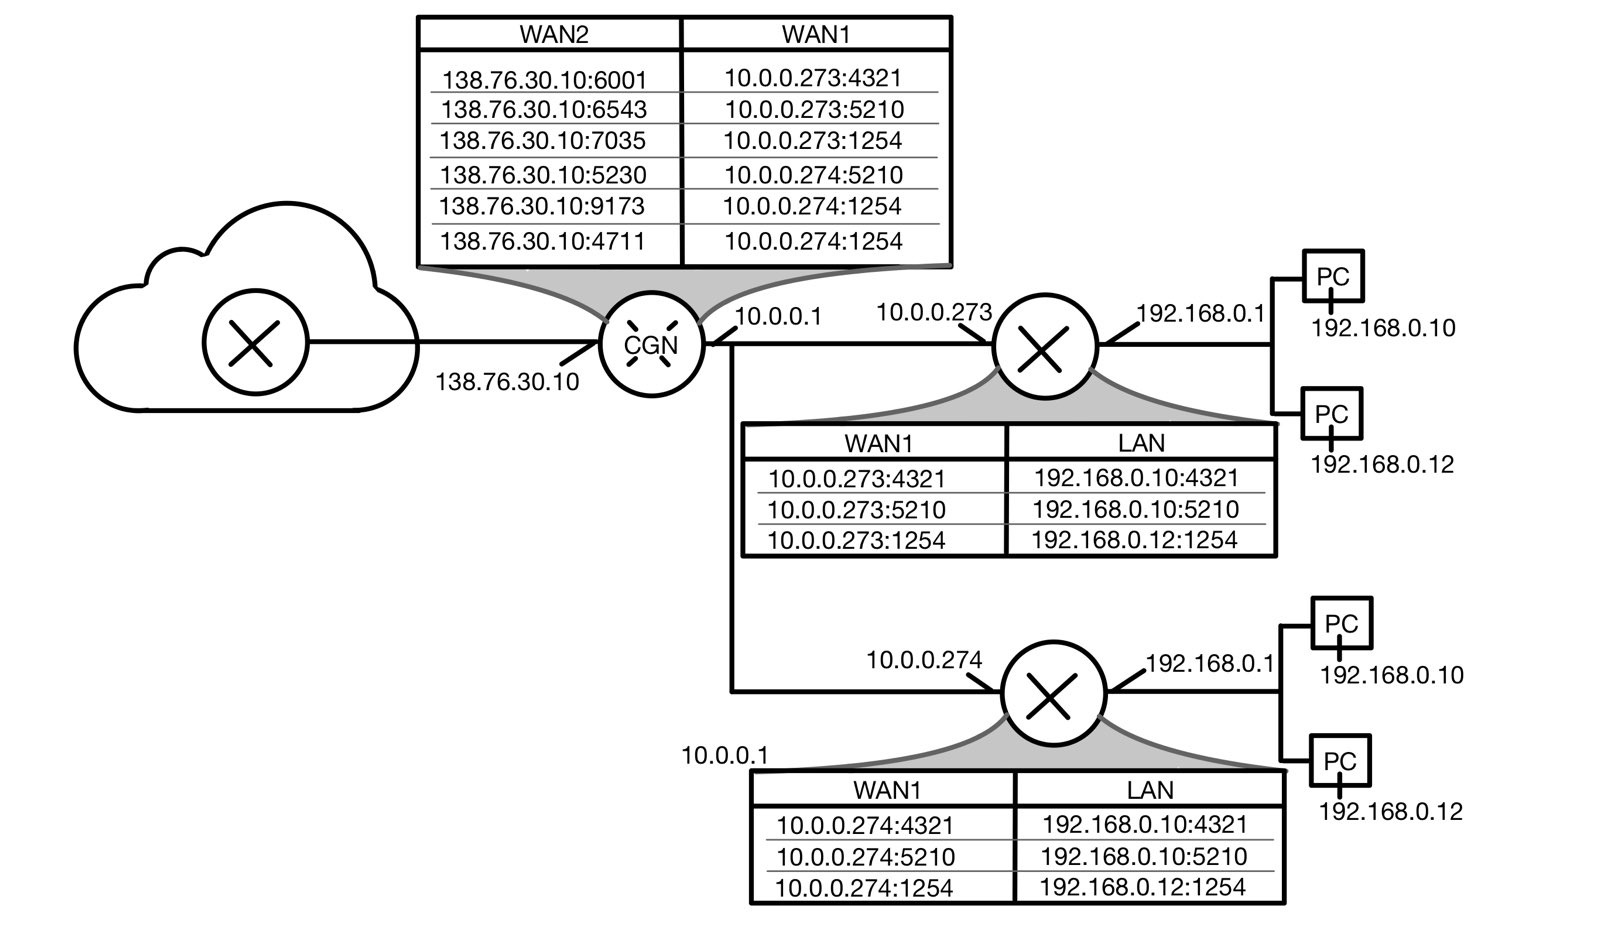
\includegraphics[width=0.5\textwidth]{images/nat_444.png}
        \caption{Example of NAT444 with translation tables}
        \label{fig:nat_444}
    \end{figure}
    In example \ref{fig:nat_444} two end-users are connected to the CGN. The CGN has the public, globally routable IPv4 \textit{138.76.30.10}. One customer gets assigned the private IPv4 \textit{10.0.0.273} and the other one the private IPv4 \textit{10.0.0.274}. Both operate a typical \textit{192.168.0.0/16} Network. As you can see, both customers have a personal computer with the private IPv4 \textit{192.168.0.10}. Yet the system works. After the end-user NAT translation, these personal computers have the IPv4 \textit{10.0.0.273} and \textit{10.0.0.274} with the corresponding ports. Then the CGN translates these private IPv4 addresses into the only public, globally routable IPv4 \textit{138.76.30.10}. The CGN translates IP and Port and maps them to the corresponding customer. In a real world application, the CGN would control multiple public, gloablly routable IPv4 addresses and split them between all customers. Example \ref{fig:nat_444} only shows a cutout of the whole CGN\cite{Hughes2022_C11}.
    \subsection*{END-USER IMPACT}
    NAT44, A+P and NAT444 cause very similar problems and have a huge impact on the end-user. Some of them will be discussed now.\\\\The first problem is regarding location services. Typically it is possible to determine a rough geo-location regarding one single public IPv4. Especially with NAT444 one IPv4 is shared by many users. Thus it is not really possible to accurately guess the location. Some people might argue that this is a advantage too, because it increases privacy\cite{Hughes2022_C04}.\\\\A very serious problem is regarding spam. IPv4 addresses which are distributing spam, typically can be blacklisted. With a shared IPv4 address between multiple end-users this can lead to blocking of innocent end-users who just were unlucky to share a IP with an adversary\cite{Hughes2022_C04}.\\\\Another problem is regarding peer-to-peer applications. To establish and maintain a peer-to-peer network it is necessary to ping a peer directly. This happens with a public IPv4 and a well known port. With NAT that is generally not possible. All devices share one IPv4 with all ports\cite{Hughes2022_C04}.\\\\Similar to peer-to-peer it is not possible to host own servers behind a NAT. Web servers for example establish \textit{https} connection over the well-known port \textit{443}. With NAT44 it is theoretically possible to forward a port to one device. Thus it is possible to operate one server of a kind per port. For example one web server and one ftp server. With A+P or NAT444 this option is completely gone and it is not possible to host servers. That impacts end-users massively. The main idea of the internet is a decentralised network. Everyone should be able to set up servers and start communications without a central instance. NAT disabled this main idea of the internet\cite{Hughes2022_C04}.\\\\Modern web applications nowadays usually require many ports to operate. With NAT these ports are limited and could run short. This is a very serious problem, because as it is not possible to create more IPv4 addresses, it is not possible to create more Ports\cite{Hughes2022_C04}.\\\\Apart from the obvious disadvantages, some protocols like DNS are less secure with NAT. Because of the \textit{DNS poisoning attack}, a client starts new DNS requests with a random port. Assuming that an attacker cannot guess the port, the DNS server answers to that port. If an attacker can guess the port and answer to it first, the attacker can infiltrate wrong DNS entries. This is a serious security risk. With the use of NAT44 all devices share the available ports. The problem gets even worse with A+P or NAT444. If an attacker knows the assigned port range, the DNS cache poisoning attack is very effective. IPSec needed to be upgraded to work with NAT44 and currently does not work with NAT444\cite{Hughes2022_C04}.\\\\A general problem with NAT is, that it is a single point of failure. If a personal NAT router or a CGN router is not working anymore, all clients cannot access the internet. A NAT router is a very lucrative attack target\cite{Hughes2022_C04}.\\\\In a nutshell, NAT has many problems. It was meant as a quick fix until the next generation of IP is finalized. Unfortunately, NAT outlived it supposed lifetime by many years. This is why modern solutions are required to get away from NAT and return to the original open and accessable internet.
    \section{MODERN SOLUTIONS}
    It became very clear that IPv4 is not sufficient anymore. This is why IPv6 was standardized. IPv6 addresses are a \textit{128} bit string. With IPv6 it is possible to assign $2^{128}=3.4*10^{38}$ addresses. This number of addresses will suffice forever. IPv6 indefinitely solves the IPv4 exhaustion problem. Unfortunately IPv6 is not backwards compatible to IPv4. The first solution was to implement IPv6 alongside IPv4. This gives older applications the possibility to continue using IPv4 until they and the servers are upgraded. Assigning both an IPv4 address and IPv6 addresses is called \textit{dualstack}. The two very similar technologies \textit{dualstack} and \textit{dualstack lite} are introduced now. They are meant to be transition technologies from the world of IPv4 only to IPv6 only.
    \subsection{DUALSTACK}
    With \textit{dualstack} the end-user gets a public, globally routable IPv4 address and a block IPv6 addresses from the ISP. With the IPv4 address, the end-user performs NAT44. This was discussed in the previous chapter. In addition to that private IPv4 address, all devices also get assigned a global, publicly routable IPv6 address \cite{8716482}. A personal computer now has two implemented IP layers as in \ref{fig:dualstack}. Old application that only support IPv4 work seamlessly without any modification required.
    \begin{figure}
        \centering
        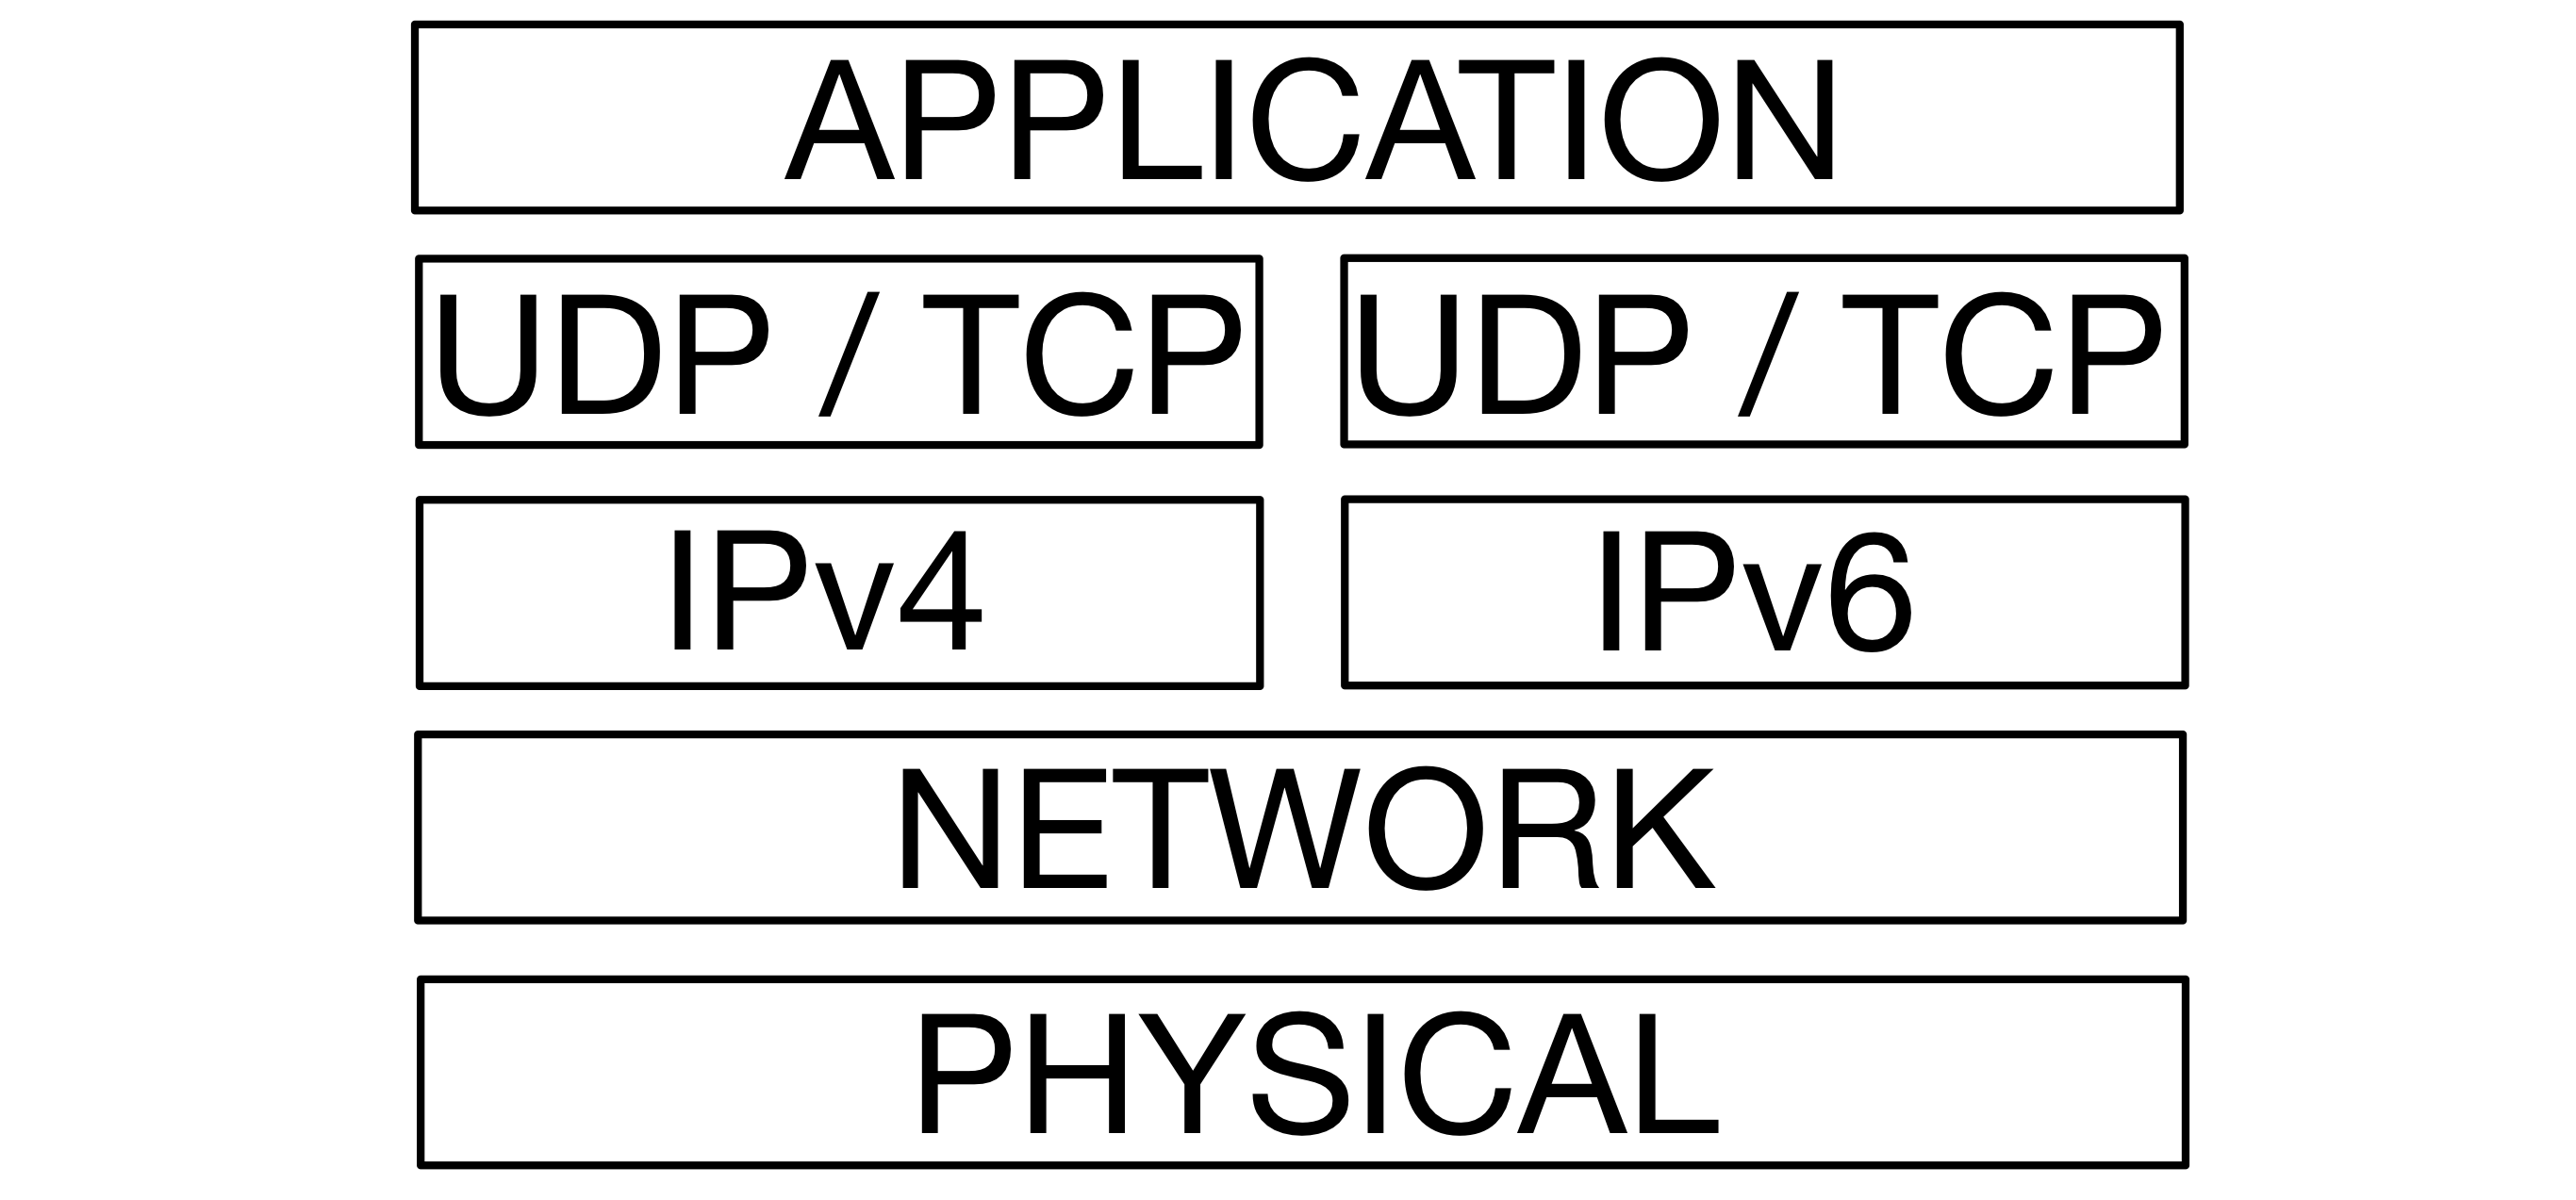
\includegraphics[width=0.5\textwidth]{images/dualstack.png}
        \caption{Dualstack IP layer implementation}
        \label{fig:dualstack}
    \end{figure}
    With IPv6 an ISP typically get a \textit{/32} network containing $2^{128-32}=2^{96}$ IPv6 addresses. The end-user then gets a \textit{/64} network. IPv6 addresses are noted as 8 two byte blocks divides by a colon. The example in \ref{fig:dualstack_network} shows a very basic end-user \textit{dualstack} network containing one router and two end-devices. The ISP got the \textit{2001:0db8:0000:0000:0000:0000:0000:0000/32} block assigned. The router implements NAT44 and got the block \textit{2001:0db8:0001:0002:0000:0000:0000:0000/64} assigned by the ISP. The router can now distribute the last 4 two byte blocks to the devices. In this example the two personal computers got the public, globally routable IPv6 \textit{2001:0db8:0001:0002:0000:0000:0000:0010} and \textit{2001:0db8:0001:0002:0000:0000:0000:0012}. In addition to that the router assigns the private IPv4 addresses \textit{192.168.0.10} and \textit{192.168.0.12} to the personal computers. An application on one personal computer can now use the private IPv4 address with all the disadvantages discussed earlier or use the IPv6 address.
    \begin{figure}
        \centering
        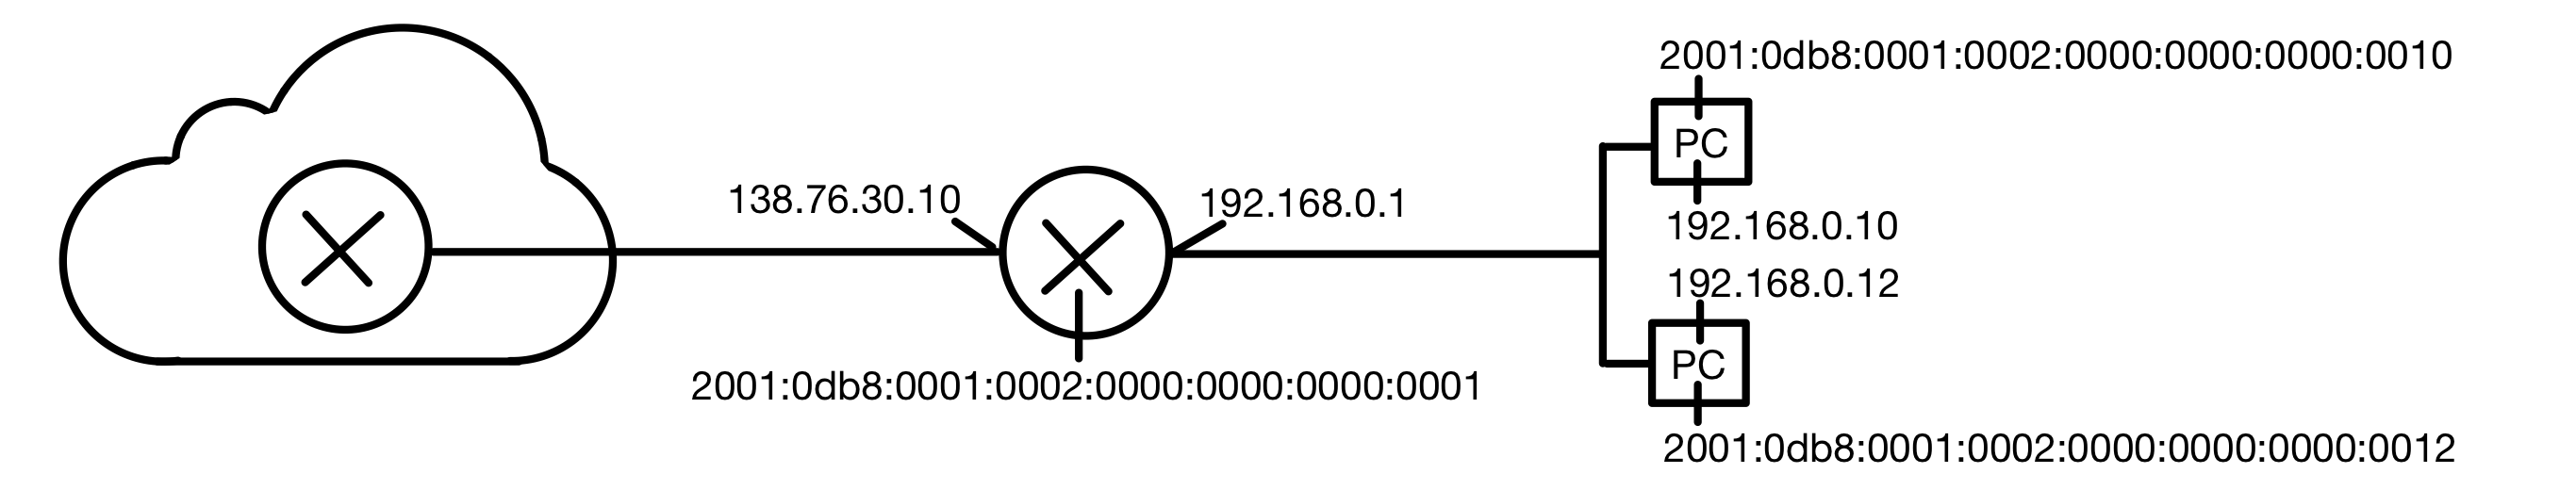
\includegraphics[width=0.5\textwidth]{images/dualstack_network.png}
        \caption{Example of a Dualstack network}
        \label{fig:dualstack_network}
    \end{figure}
    \subsection{DUALSTACK LITE}
    \textit{Dualstack Lite} also called \textit{DS Lite} is similar to \textit{dualstack} from a end-device point of view. An end-device gets a public, globally routable IPv6 address and a private IPv4 address. The end-device needs an \textit{dualstack} implementation as shown in \ref{fig:dualstack}. In case the device wants to communicate with an IPv4 legacy server, the device has to use the IPv4 stack and the private IPv4. In all other cases the public, globally routable IPv6 is preferred. There is no translation between IPv4 and IPv6 or the other way around. All in all \textit{dualstack} and \textit{dualstack lite} does not differ for the end-device.\\\\Compared to \textit{dualstack}, the network traffic between the router of the customer and the ISP is IPv6 only. IPv4 packets are tunneled in IPv6. The IPv4 packet is part of the data field of the IPv6 packet. DNS is done over IPv6 only. The \textit{B4} element will perform DNS for all clients in the network. Thus DNS is never routed to \textit{AFTR}.\\\\ \ref{fig:dualstack_lite_network} is an example of a basic \textit{dualstack lite} setup. The customers router has a \textit{B4} element. This \textit{B4} element directly connects to the ISPs \textit{AFTR}. The \textit{B4} and \textit{AFTR} create an IPv6 tunnel for IPv4 packets. NAT44 is only applied at ISP level. Though, each customer hosts his own DHCPv4 Server to distribute IPv4 addresses in the home network. The IPv4 packets are packed into the IPv6 data field and directly send over IPv6 to the \textit{AFTR}. The \textit{AFTR} receives the IPv6 packages and extracts the IPv4 packages. Now the AFTR does NAT44. In addition to the original private IPv4 address and the port, the NAT table also saves the assigned IPv6 block for the customer. Because of that, the end-user can theoretically use an arbitrary private IPv4 block\cite{rfc6333}. \ref{fig:dualstack_lite_network} shows that \textit{customer 1} and \textit{customer 2} both use the private IPv4 block \textit{192.168.0.0/16}. There are even two personal computer with both the private IPv4 \textit{192.168.0.12} in combination with the port \textit{3872}. This is no problem, because the NAT table also stores the customer assigned IPv6 block. \textit{Dualstack Lite} allows nearly endless scaling. It is not necessary to assign one public IPv4 per costumer. Over the time, the workload for the NAT table will decline because more and more clients will use the superior public, globally routable IPv6 address. There are only two cases, when IPv4 is needed. Either a legacy IPv4 application or device on the client side, or a device that wants to reach a server that is only recable over IPv4.\\\\\textit{Dualstack lite} also works with IPv4 only and IPv6 only devices. These only get assigned the corresponding IP address and work as intended. \textit{Dualstack lite} only uses NAT44 similar to \textit{dualstack}. That is why both are superior to \textit{NAT444}, while providing a usable solution even with IPv4 exhaustion\cite{Hughes2022_C08}.
    \begin{figure}
        \centering
        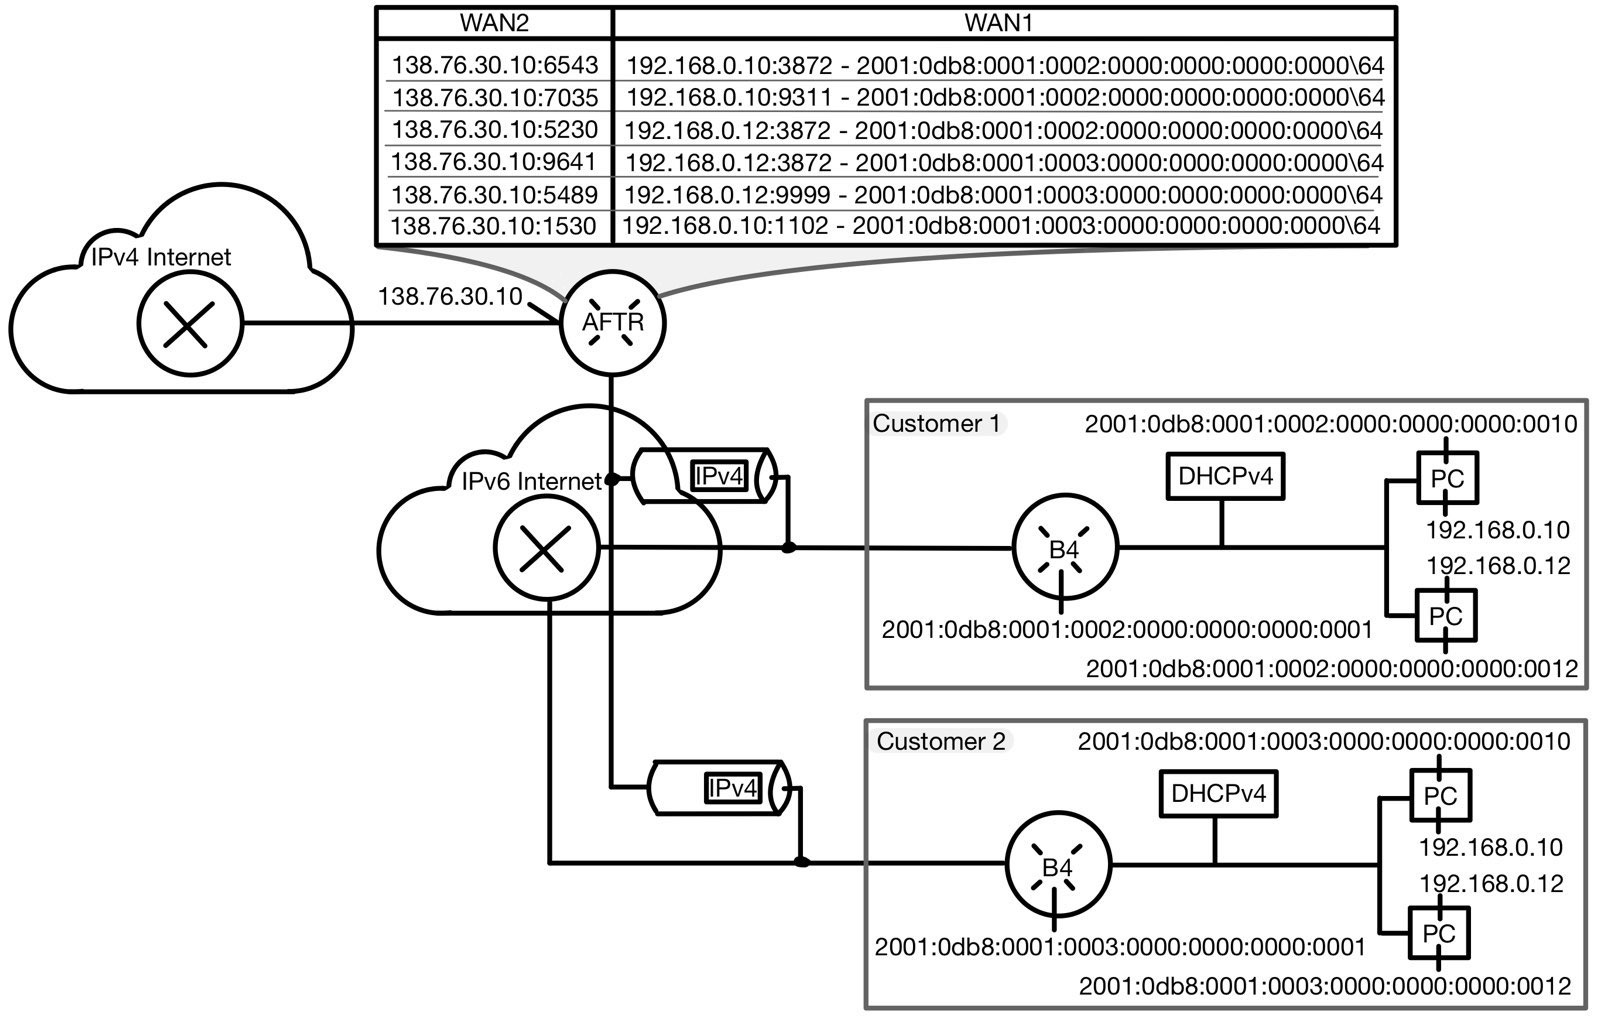
\includegraphics[width=0.5\textwidth]{images/dualstack_lite_network.png}
        \caption{Example of a dualstack Lite network}
        \label{fig:dualstack_lite_network}
    \end{figure}
    \subsection*{END-USER IMPACT}
    \textit{Dualstack} and \textit{dualstack lite} provide the first real solution to the IPv4 exhaustion problem. They use IPv6 addresses. IPv6 addresses enable the end-user for the first time to get public, globally routable IP addresses for all their devices. This has many advantages but some disadvantages too. These will be discussed now.\\\\The introduction of IPv6 partially solves the NAT44 and NAT444 problem. Protocols like IPSec or peer-to-peer protocols function out of the box, without any server, protocol extension or additional setup. IPv6 does not provide any NAT functionality and will never need it.\\\\Because each device has a unique IPv6 address, all ports are available for that device. Modern and future port intensive applications work without a problem.\\\\IPv6 enables new multicast and broadcast features. With \textit{dualstack}, customers can experience IPTV seamlessly over IPv6 and benefit from the new features. VoIP also works better with IPv6. \\\\IPv6 enables end-to-end connectivity. This opens up better gaming multiplayer performance. Gamer do not have to care about different NAT types anymore.\\\\With direct true end-to-end TLS communication, a trusted channel between to parties can be established without a server and with use of client TLS certificates. This opens up new innovation possibilities for messager-apps and much more.\\\\The introduction of IPv6 to end-users with \textit{dualstack} and \textit{dualstack lite} has some downsides too. The main problem is regarding privacy. This will be discussed later on in this paper. \textit{Dualstack} and \textit{dualstack lite} have a security problem that is not related with IPv6 directly. Most devices accept IPv4 and IPv6 traffic. This leads to many firewall rules. System administrators and especially end-users can make many mistakes setting up the system. This can lead to exposed clients which are reachable over the internet even though they should remain private.\\\\All in all, \textit{dualstack} and especially \textit{dualstack lite} are the first good solutions for the IPv4 exhaustion problem. Apart from a more complicated and complex setup, the end-user can use new features and capabilities to explore the internet. \textit{Dualstack} is the first step in the direction to return the internet to an open and accessible global network where everyone can host servers and access content.
    \section{LATEST SOLUTION: IPv6 ONLY}
    Unfortunately \textit{dualstack} still requires the assignment of one or multiple IPv4 addresses per user. ISPs, especially mobile internet providers, run out of IPv4 addresses and want to transition to the new technology IPv6. This is mainly to reduce complexity and cut costs. That is why ISPs start to roll out IPv6 only connections. The end-user usually gets one \textit{/64} IPv6 block.\\\\If the end-user only accesses IPv6 content no problems appear. In case a end-device wants to access an IPv4 only server, network-based translation is required. Another problem occurs regarding IPv4 legacy applications that run on IPv6 only end-devices. These IPv4 requests must be translated too. This happens on the end-device itself with host-based translation. In the following network-based translation performed by the ISP and host-based translation performed by the end-devices will be discussed.
    \subsection{NETWORK-BASED TRANSLATION: NAT64/DNS64}
    \textit{NAT64} in combination with \textit{DNS64} is a way for ISPs to deploy IPv6 only to their customers. \textit{NAT64} only works if all end devices support IPv6 natively. This is the case for nearly all devices. Every device from the end-user gets a public, globally routable IPv6 address. If a device wants to connect to a website, the URL is translation to an IP address with the use of the \textit{Domain Name System} or short \textit{DNS}. \textit{DNS} works a little bit different in this setup. The default \textit{DNS} server is not a normal DNS server, but a special \textit{DNS64} server. The \textit{DNS64} server works as the following.\\\\First the \textit{DNS64} server forwards the request to a normal \textit{DNS} server. This normal \textit{DNS} server can be reached either over IPv4 or IPv6. In example \ref{fig:nat_64_dns_64} the \textit{DNS} server is reached over IPv4. If the \textit{DNS} server delivers a AAAA record for the requested domain, the end-user client communicates normally over IPv6. If the \textit{DNS} server only delivers an A record for the domain, the \textit{DNS64} manipulates the DNS record and delivers an AAAA record with a special IPv6 address to the client. The special address points to the ISP's \textit{NAT64} endpoint. The address of the \textit{NAT64} server consists of two parts. The first part is a well-known standardized part to reach the \textit{NAT64}.
    \begin{center}
        0064:ff9b::/96
    \end{center}
    The second part encodes the original requested 32-bit IPv4 address. Both parts are combined as described in RFC6052 \cite{rfc6052}. In the example \ref{fig:nat_64_dns_64}, the server \textit{example.com} only accepts IPv4 traffic. Thus the \textit{DNS} server only return an A record with the public IPv4 address \textit{192.0.2.33}. The \textit{DNS64} manipulates that record and returns an AAAA record with the IPv6 address \textit{0064:ff9b:0000:0000:0000:0000:c000:021}. The first part is the standardized prefix. The second parts looks a little bit different than the IPv4 address. Each of the four IPv4 address parts, that is represented by a number between 0 and 255, is represented by two hex digits now. The first block \textit{192} is represented as a \textit{c0} in hex. The second block \textit{0} is represented as a \textit{00} in hex. The third part \textit{2} as a \textit{02} in hex and the last part \textit{33} as a \textit{21} in hex\cite{rfc6052}.\\\\A client device that wants to access an IPv4 server sends IPv4 packages according to the \textit{DNS64} AAAA record. The ISP's \textit{NAT64} server gets these IPv6 packages and translates them into IPv4. A NAT translation is performed. The \textit{NAT64} server maps its public IPv4 address and a certain port to the IPv6 address plus port. This is similar to a \textit{NAT44} translation. The IPv4 only server does not notice that the connection is between an IPv6 and IPv4 device.\\\\It is only possible to establish an connection from an IPv6 device to and IPv4 device. This direction works, because the IPv6 address is four times longer than the IPv4 address. The IPv4 and the \textit{NAT64} server can be encoded into one address as decrebed above. It is not possible to encode an IPv6 address into IPv4. The only possibility to start an IPv4 to IPv6 conenction is over static routes. The \textit{NAT64} would have to assign a public IPv4 to an IPv6 exclusively. This eliminates the benefit of IPv6 and is not possible on a scale due to IPv4 exhaustion\cite{rfc6146}.
    \begin{figure}
        \centering
        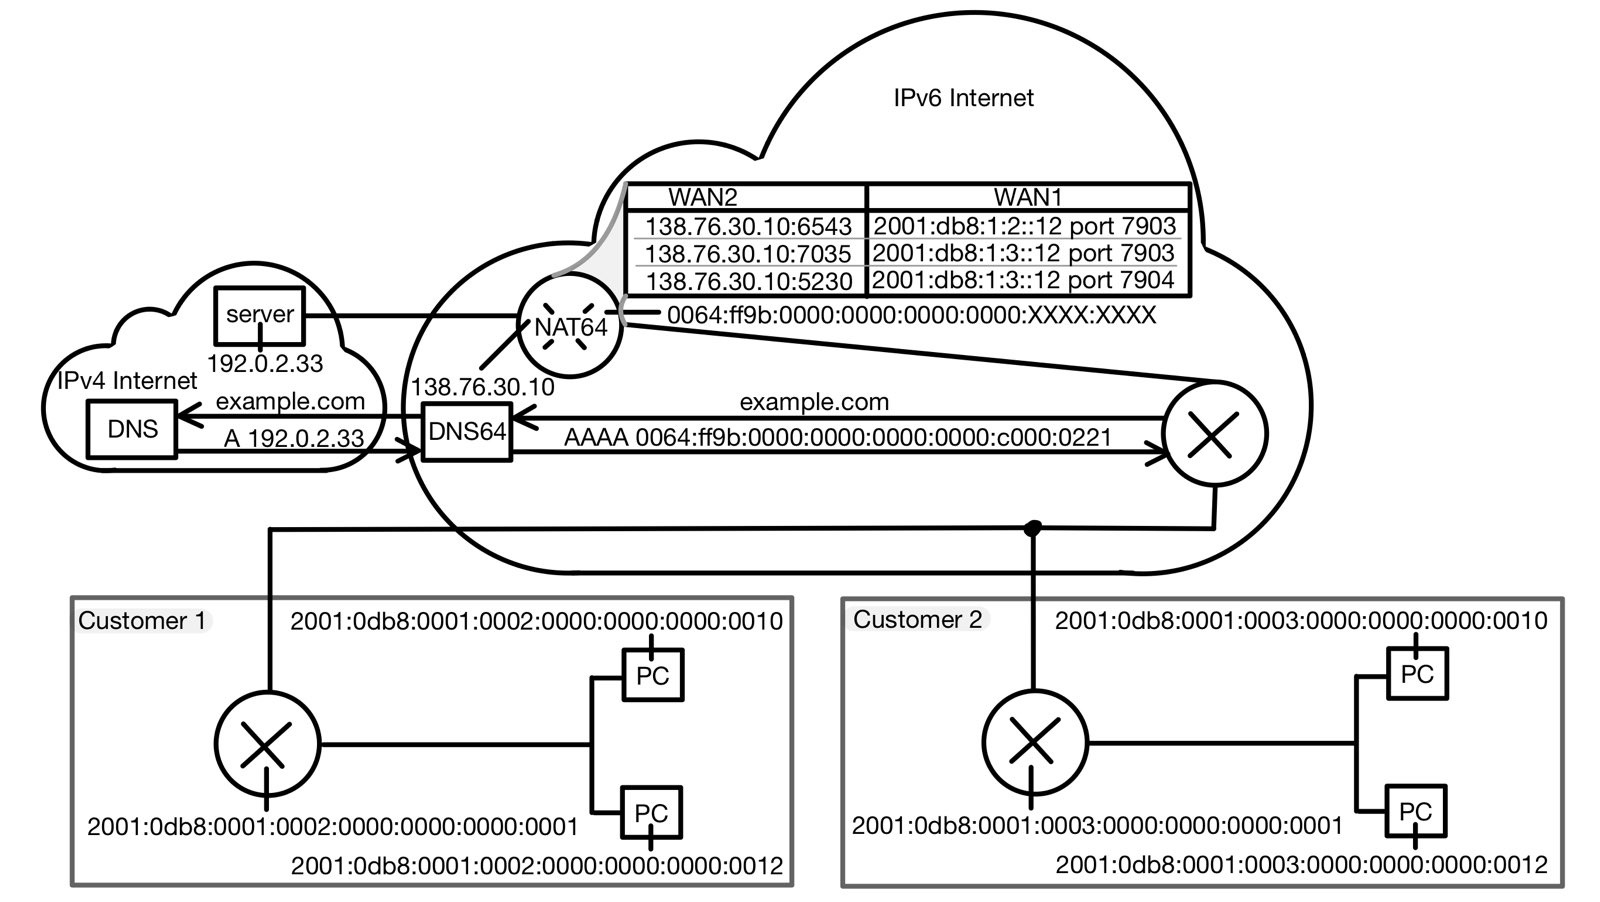
\includegraphics[width=0.5\textwidth]{images/nat_64_dns_64.png}
        \caption{Example of a NAT64/DNS64 network}
        \label{fig:nat_64_dns_64}
    \end{figure}
    \subsection{NETWORK-BASED TRANSLATION: 464XLAT}
    \textit{464XLAT} as described in the RFC \cite{rfc6877} is a combination of stateful and stateless translation. The ISP only provides an IPv6 connection to the customer. All ISP internal networks can be IPv6 only. Each end-device can get an private IPv4 and a public IPv6 address. It is possible that some devices only get IPv4 addresses and others only get IPv6 addresses. There are two translators involved.\\\\The first translator is at customer-side. It is called \textit{CLAT}. The \textit{CLAT} performs a stateless translation, which translates a private IPv4 address into a public IPv6 address. This is a bijective one to one mapping and therefore stateless. The \textit{CLAT} also performs routing, DNS and acts as a DHCP server. It is a usual home router.\\\\The second translator is at ISP side. It is called \textit{PLAT}. The \textit{PLAT} is stateful and translates global IPv6 addresses to global IPv4 addresses. It works like a NAT64 as described above.\\\\\textit{464XLAT} only works with a typical client-server model where the server has a public, globally routable IPv4 address. Inbound IPv4 connections to the customer are not possible. There are three different ways of communication.\\\\The first option for a device is to use it's public, globally routable IPv6 address to directly communicate with other IPv6 capable devices. No translation is required. All IPv6 features work as intended, because IPv6 is directly used.\\\\The second option is to connect from an IPv6 end-device to an IPv4 server. This is done with a stateful translation, performed by the \textit{PLAT} at the provider. This is equivalent to \ref{fig:nat_64_dns_64}. A \textit{NAT64} is used.\\\\The third option is to connect from a IPv4 end-device to a IPv4 server. This uses both, the client side \textit{CLAT} and the ISP side \textit{PLAT} and is the actual \textit{464XLAT}. First the private IPv4 address of a end-device is uniquely mapped to a Public IPv6 address. This is done similar to \textit{DNS64} but with an /64 block. The exact mapping is defined in RFC6052 \cite{rfc6052}. The most important property is, that it is a bijective and stateless. The \textit{PLAT} of the ISP is reached over IPv6. Then the \textit{PLAT} translates the IPv6 address with \textit{NAT64} to an public IPv4 address. The client using a private IPv4 address now communicates over IPv6 with another IPv4 only server. A end-user can use their home setup with private IPv4 addresses as usual. \textit{464XLAT} translates everything to IPv6 and back to IPv4.This is desirable for the provider, because the ISP can deploy IPv6 in their entire network and only needs a \textit{PLAT} at the edge to a connecting IPv4 network.\\\\It is important to note that it is not possible to reach an IPv6 client from an IPv4 end-device. This is an expected behaviour and not a problem. Most IPv6 servers are dualstack and also support IPv4.
    \begin{figure}
        \centering
        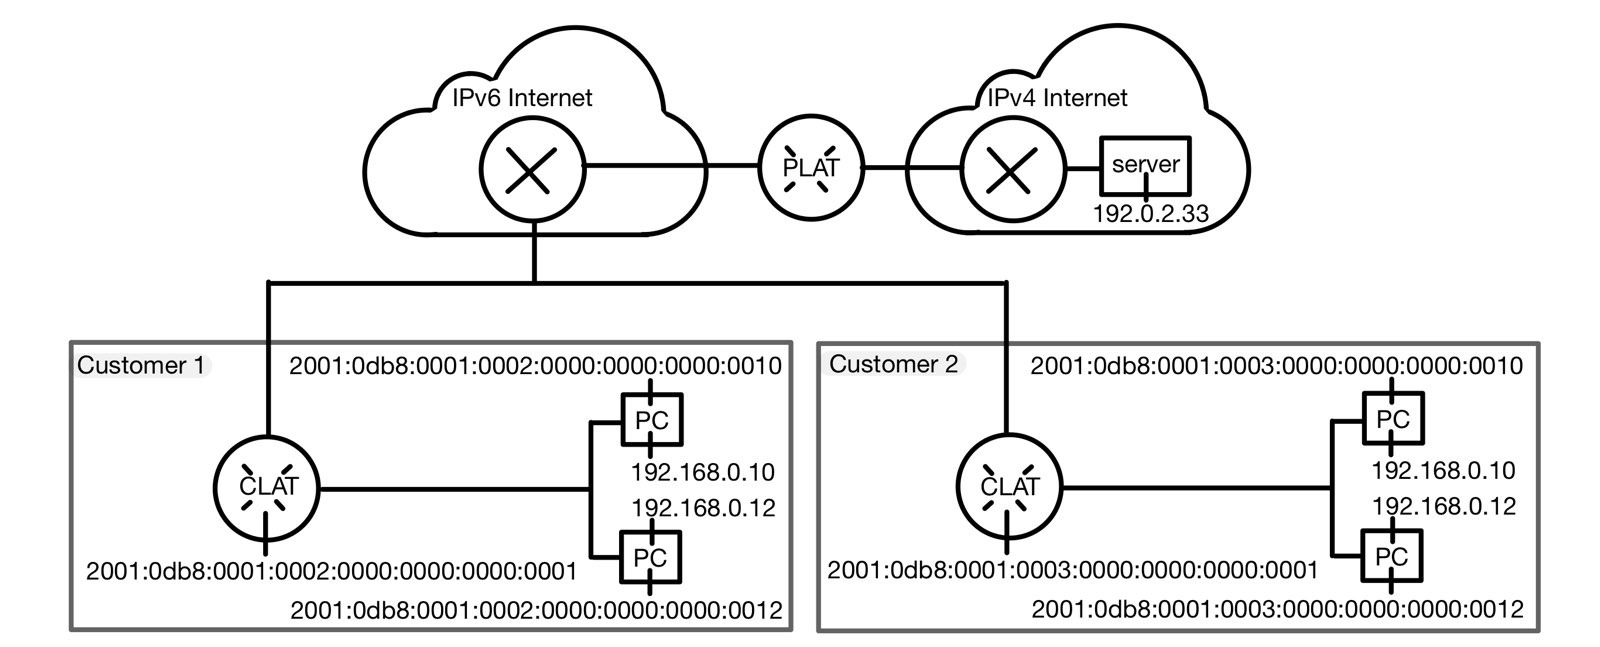
\includegraphics[width=0.5\textwidth]{images/464_xlat.png}
        \caption{Example of a 464XLAT network}
        \label{fig:646_XLAT}
    \end{figure}
    \subsection*{END-USER IMPACT: NETWORK-BASED TRANSLASTION}
    \textit{NAT64} in combination with \textit{DNS64} or \textit{464XLAT} has great advantages for the ISPs. It enables them to completely switch to IPv6 on their internal network and still provide legacy IPv4 support for their costumers. The end-user experiences some advantage and some disadvantages with a network based translation which will be discussed now.\\\\The end-user profits from native IPv6 support. Once the transition is completed, neither the ISP nor the end-user needs to do much. The \textit{DNS64} and \textit{NAT64} servers can be deactivated or kept online for a very small number of still present IPv4 servers. The end-users can keep using their network equipment. If \textit{464XLAT} is used, the user could do an update and only use IPv6 in the future, eliminating all private IPv4 address in the network. With \textit{NAT64}, IPv6 is already used exclusively. This simplifies the setup. It increases security too, because only one set of firewall rules needs to be set. A simpler setup is more error-resistant and thus more secure. Being future-proof is an advantage for the end-user too.\\\\\textit{NAT64} has some disadvantages for the end-user. A special \textit{NAT64} is used. DNSSEC does not work, because \textit{NAT64} manipulates the records. That is what DNSSEC tries to prohibit. Moreover, it is not possible to establish a connection from an IPv4 only device to the home network of the end-user. The end-user can only host servers for IPv6 devices. This is a clear drawback, compared to \textit{dualstack}. With \textit{dualstack} and port-forwarding, at least one server per port can be hosted. This disadvantages is less dramatic, the more the IPv6 transition continues. I assume that most end-user try to access their home devices from a mobile device. Nearly all mobile devices support IPv6 by default. Many protocols that embed the IP address at higher levels will probably not work, because a NAT is used for translation. It is desirable to complete the IPv6 transition as fast as possible to end the use of NAT indefinitely. Translation in general also effects the performance of devices. IPv6 only users are negativly effected by translation\cite{10.1109/TNET.2015.2453338}. Devices with a static IPv6 address can easily be tracked. Normally the device MAC-Address is used as a suffix for the last blocks of the IPv6 address. IPv6 can be a privacy problem. There a ideas to randomise the IPv6 address on the end-device to improve privacy. This is a problem that can be fixed.
    \subsection{HOST-BASED TRANSLATION: BIS}
    \textit{Bump-In-the-Stack} or short \textit{BIS} is a technique that allows IPv4 legacy applications on a \textit{dualstack} device to communicate with an IPv6 host over IPv6. This only works when the legacy application wants to reach a sever over a URI. It does not work with embedded IPv4 addresses. The request is intercepted between the TCP/IP or UDP/IP module and the network card driver. The data is extracted and packed in to an IPv6 package. The corresponding IPv6 address is found with a DNS request. This only works on dualstack end-devices because an IPv4 stack is needed. The translation happens afterwards\cite{8716482}.
    \subsection{HOST-BASED TRANSLATION: BIA}
    \textit{Bump-In-the-API} or short \textit{BIA} is a similar technique. It also only works on dualstack end-devices. The socket call is intercepted. Instead of an IPv4 socket call, an IPv6 socket is invoked. This also does not work with hard-coded IPv4 addresses\cite{8716482}.
    \subsection{HOST-BASED TRANSLATION: BIH}
    \textit{Bump-In-the-Host} or short \textit{BIH} combines \textit{BIS} and \textit{BIA}. With \textit{BIH} it is possible to support an IPv4 only legacy application on an IPv6 only device. Thus it is possible to run these application when an IPv6 only connection is provided by the ISP. This also requires a name based connection and not a embedded IPv4 address\cite{8716482}. 
    \subsection*{END-USER IMPACT: HOST-BASED TRANSLATION}
    Host-based translation is the last puzzle peace for an IPv6 only system. Network-based translation enables users to deploy an IPv6 only network at their home. This requires all end-devices to support IPv6. In addition to that, all applications running on these end-devices need to support IPv6 too. Most applications probably automatically support IPv6 because they are programmed in a higher level programming language. Specific legacy low-level IPv4 only applications might not support IPv6 out of the box. Host-based translation enables end-users to continue using these applications. Multicast and embedded addresses are not supported. The end-user could experience rare situations where programs will not work. Host-based translation in general only has positive effects for the end-user, because it enables nearly all IPv4 only applications to run.
    \section{ISP Tunnels}
    This last section deals with ISP tunnels. Especially at the beginning of IPv6 deployment, IPv6 path stability was worse than IPv4 path stability\cite{7119767}. That is because of the way ISPs transport IPv6 traffic. This has an impact on end-users. ISPs could build an IPv4 only and an IPv6 only infrastructure. To make the transition faster, ISPs tunnel IPv6 traffic over existing IPv4 paths. There are many protocols to achieve that. It is also possible to tunnel IPv4 over IPv6. Existing IPv4 dominance does not hinder IPv6 only investments because of that. In the following, two protocols of IPv6 in IPv4 tunneling will be discussed.
    \subsection{6in4 TUNNELING}
    \textit{6in4} is described in the corresponding RFC\cite{rfc4213}. The basic concept is fairly simple. The IPv6 header, the transport layer header and the data of the IPv6 packet are inserted into the data field of the IPv4 packet. Both ends of the IPv4 tunnel need public, globally routable IPv4 addresses. At the tunnel entry, the IPv6 package is encapsuled into the IPv4 package. At the tunnel exit, the IPv6 package is extracted from the IPv4 data field. The tunnel counts as a single hop regarding IPv6, regardless of the actual IPv4 hops.
    \subsection{6rd RAPID DEPLOYMENT}
    \textit{6rd Rapid Deployment} is an extension to \textit{6in4}. It allows ISPs to limit the 6in4 tunnel to their own network. Thus they can provide access to all nodes in their network and guarantee good service.
    \subsection*{END-USER IMPACT}
    Tunneling IPv6 traffic enables ISPs to rapidly provide IPv6 traffic to all customers without investing heavily in new hardware. This accelerates IPv6 adaption. With IPv6 tunneling more IPv6 paths are virtually created. Existing IPv4 paths can be used for IPv6. The end-user experiences a stable internet connection even when some IPv6 paths are not active due to technical problems. ISP tunnels have a minor effect on the end-user and will not be discussed in more detail in this paper.

    \section{Summary}
    With the exhaustion of IPv4 addresses, ISPs are now forced to transition to IPv6 addresses. This has an direct impact on the end user, because both protocols are not compatible.\\\\Before transitioning to IPv6, ISPs invested heavily in NAT systems. This caused customer end-devices to not be routable in the public internet. \textit{NAT44} effected many protocols and required a new version of them. NAT traversal can be a security problem. This is why NAT should be abandoned as soon as possible. With \textit{NAT444} even more problems appeared for the end-user.\\\\\textit{Dualstack} introduced IPv6 addresses to end-users for the first time. This enabled user to host multiple public, globally routable servers from their home. With a further scarcity of IPv4 addresses, \textit{dualstack lite} was introduced. \textit{Dualstack lite} outsources the NAT from the end-user to ISP level. The end-user can only profit from a \textit{dualstack} connection. There are only added features.\\\\Today, ISPs start to provide IPv6 only services. With \textit{NAT64/DNS64} end-users are only provided one IPv6 block. Connections to IPv4 only servers are done over ISP site translation. \textit{464XLAT} performs stateless translation at end-user level and stateful translation at ISP level. Both systems allow the ISP too share precious public IPv4 addresses among multiple customers. In most cases these IPv4 addresses are not needed, because the end-users use a native IPv6 connection to the servers they want to access. Directly compared to \textit{dualstack}, IPv6 only solutions are worse for the end-user. Translation is slower than a direct connection and some features of IPv4 do not work. It is not possible to reach an IPv6 only connected home over IPv4.\\\\With IPv6 addresses for every device, applications running on the users end-device need to support IPv6 too. \textit{Bump-In-the-Host} is a system, to use IPv6 even with legacy application that only support IPv4. Making old applications work with IPv6 has only a positive impact for the end-user\\\\To improve IPv6 availability, ISPs tunnel IPv6 traffic over existing IPv4 infrastructure. This has a positive effect on the path availability and thus a positive effect on the end-user experience. \textit{6in4} is a very basic protocol to establish those tunnels. \textit{6rd} is an improved version. The end-user profits from that.\\\\All in all, the deployment of IPv6 by ISPs benefits the end-user, at least in the long term. There might be some devices or applications not work properly at the beginning. Though, once the transition is completed, end-users have great possibilities. IPv6 enables all devices to initiate true end-to-end communication. End-users are able to host multiple servers and participate in peer-to-peer networks. Even in the short term, users profit from IPv6. For example, online multiplayer games work better with IPv6, because no NAT is involved. To answer the title of this paper in one sentence:\\\\The end-user impact is positive.

    %%section REFERENCES
    \bibliographystyle{plain}
    \bibliography{references}


\end{document}
